%!TEX program = xelatex

\documentclass[compress]{beamer}
%--------------------------------------------------------------------------
% Common packages
%--------------------------------------------------------------------------
\usepackage[ngerman]{babel}
\usepackage{array}

\usepackage{struktex}
\usepackage{framed}
\usepackage{amsmath}		% Paket fuer Mathemodus
\usepackage{amssymb}		% Paket fuer Mathemodus
\newcommand\scalemath[2]{\scalebox{#1}{\mbox{\ensuremath{\displaystyle #2}}}}

\usepackage{pgfplots}
\usepackage{tikz}                               % Bilder malen mit Latex (benötigt Paket pgf!)
\usetikzlibrary{angles,quotes,babel,calc,patterns,decorations.pathmorphing,decorations.markings,shapes,arrows,calc,positioning,fit,matrix,shadows,chains,spy,fadings}  % Spezielle Eigenschaften von tikz laden

\tikzset{
	arc to/.style={
		to path={
			let \p{arcto@1}=($(\tikztotarget)-(\tikztostart)$),
			\n{arcto@a}={acos(.5*veclen(\p{arcto@1})/(#1))},
			\n{arcto@s}={180 + atan2(\p{arcto@1}) - ifthenelse(\pgfkeysvalueof{/tikz/arc/large}==1,-1,1)*\n{arcto@a} + ifthenelse(\pgfkeysvalueof{/tikz/arc/ccw}==1,180,0)},
			\n{arcto@e}={      atan2(\p{arcto@1}) + ifthenelse(\pgfkeysvalueof{/tikz/arc/large}==1,-1,1)*\n{arcto@a} + ifthenelse(\pgfkeysvalueof{/tikz/arc/ccw}==1,180,0)}
			in
			\if\pgfkeysvalueof{/tikz/arc/ccw}0
			(\tikztostart) arc [start angle=\n{arcto@s}, end angle=\n{arcto@e}, radius={#1}] \tikztonodes
			\else
			(\tikztostart) arc [start angle=\n{arcto@e}, end angle=\n{arcto@s}, radius={#1}] \tikztonodes
			\fi
		}
	}
}

\newenvironment{customlegend}[1][]{%
	\begingroup
	% inits/clears the lists (which might be populated from previous
	% axes):
	\csname pgfplots@init@cleared@structures\endcsname
	\pgfplotsset{#1}%
}{%
% draws the legend:
\csname pgfplots@createlegend\endcsname
\endgroup
}%

\pgfkeys{/pgfplots/number in legend/.style={%
		/pgfplots/legend image code/.code={%
			\node at (0.125,-0.0225){#1}; % <= changed x value
		},%
	},
}

% makes \addlegendimage available (typically only available within an
% axis environment):
\def\addlegendimage{\csname pgfplots@addlegendimage\endcsname}

\usepackage[compatibility=false]{caption}
%--------------------------------------------------------------------------
% Load theme
%--------------------------------------------------------------------------
\usetheme{cats}
\usepackage{dtklogos} % must be loaded after theme

%--------------------------------------------------------------------------
% General presentation settings
%--------------------------------------------------------------------------

\title{\textcolor{RWTHblue}{\textbf{Berechnung einer Schattenprojektion}}}
\institute[FH Aachen]{\textbf{Vortrag}\\ \vspace{0.25cm} \tiny{Fachhochschule Aachen, Standort Jülich\\Studiengang: Technomathematik}
}
\author{Karsten Goebbels, Cornelia Krome, \\ Vera Loeser, Andreas Mergl}
\date{28. Juni 2016}

%--------------------------------------------------------------------------
% Notes settings
%--------------------------------------------------------------------------
%\setbeameroption{show notes}


\begin{document}
%--------------------------------------------------------------------------
% Titlepage
%--------------------------------------------------------------------------

\maketitle

%--------------------------------------------------------------------------
% Table of contents
%--------------------------------------------------------------------------
\section*{Inhalt}
\begin{frame}{Inhalt}
	% hideallsubsections ist empfehlenswert für längere Präsentationen
	\begin{minipage}{0.43\linewidth}
		\tableofcontents[hideallsubsections]
	\end{minipage}
	\hspace*{0.05\linewidth}
\end{frame}

%--------------------------------------------------------------------------
% Content
%--------------------------------------------------------------------------
\section{Motivation}
\subsection{Motivation}
\begin{frame}{Motivation}
	\begin{itemize}
		\item Entwicklung einer neuen Messtechnologie
		\item Schattenprojektion
		\item XUV-Strahlung 
		\item Genauigkeit taktiler und der Schnelligkeit optischer Messgeräte.
	\end{itemize}
\end{frame}

\subsection{Problemstellung}
\begin{frame}{Problemstellung}
		\begin{itemize}
			\item Kalibrierung: Aktivitäten zur Ermittlung des Zusammenhanges zwischen einem Messwert und der zugehörigen Messgröße
			\item kein Eingriff in die Messeinrichtung
			\item mehrere Komponenten:
			\begin{itemize}
				\item XUV-Quelle (eXtrem UtraViolette-Strahlung)
				\item Detektor
				\item Drehteller
				\item Zylinder
			\end{itemize}
		\end{itemize}
\end{frame}

\begin{frame}{Aufbau}
	\centering
	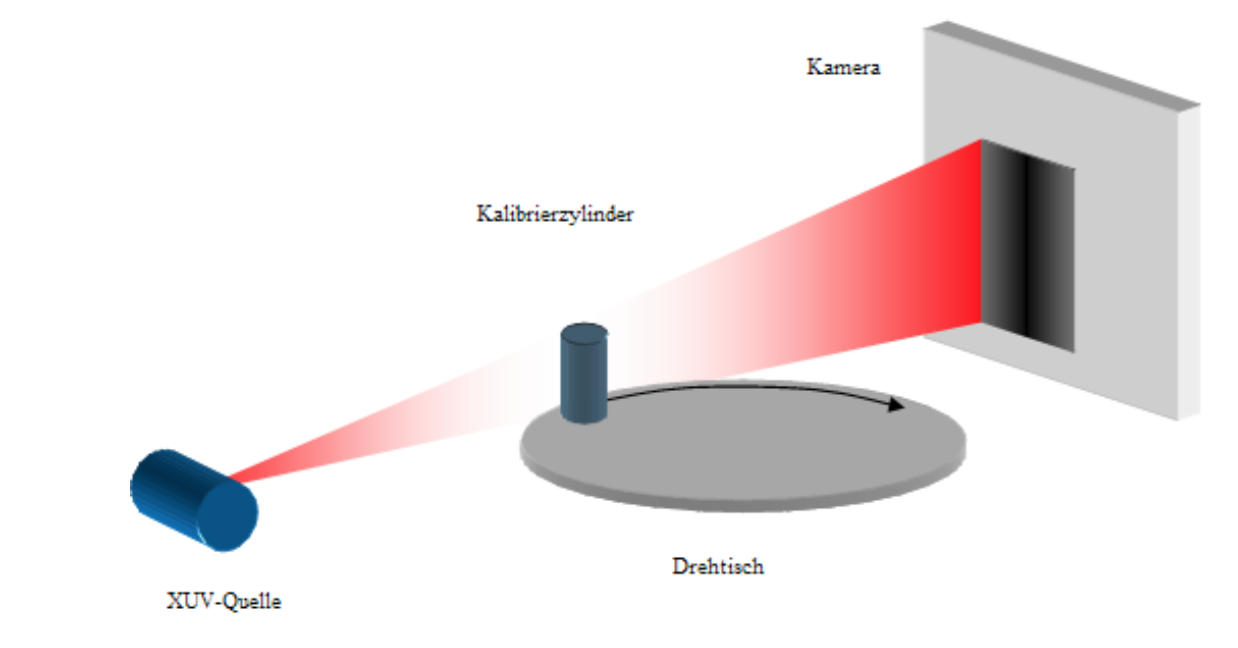
\includegraphics[width=\linewidth]{images/aufbau.png}
\end{frame}

\begin{frame}{grobe Werte}
	\centering
	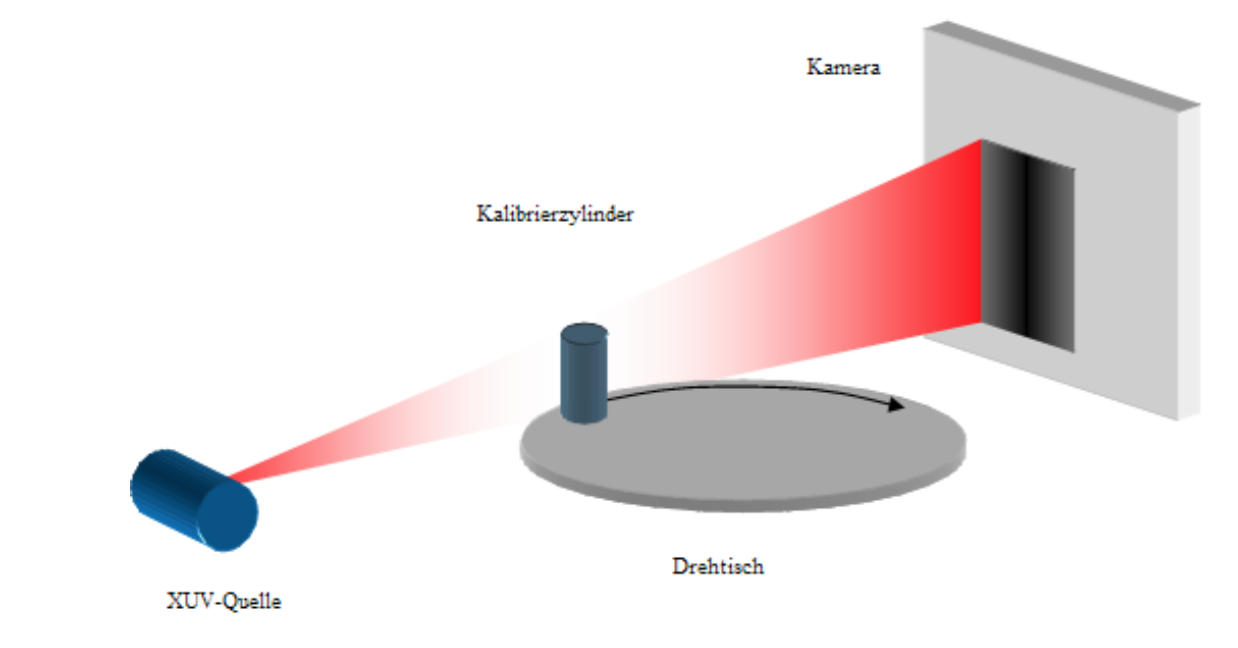
\includegraphics[width=0.5\linewidth]{images/aufbau.png}
	\begin{itemize}
		\item Radius vom Zylinder: 3~mm
		\item Radius vom Drehteller: 10~cm
		\item Abstand XUV-Quelle--Drehteller: 30~cm
		\item Abstand Drehteller--Wand: 60~cm
		\item Winkel Wand: 90$^\circ$
	\end{itemize}
\end{frame}

\section{Modellierung}
\subsection{Geometrie}
\begin{frame}{Geometrie}
	\begin{columns}
		\begin{column}{0.68\linewidth}
			\centering
			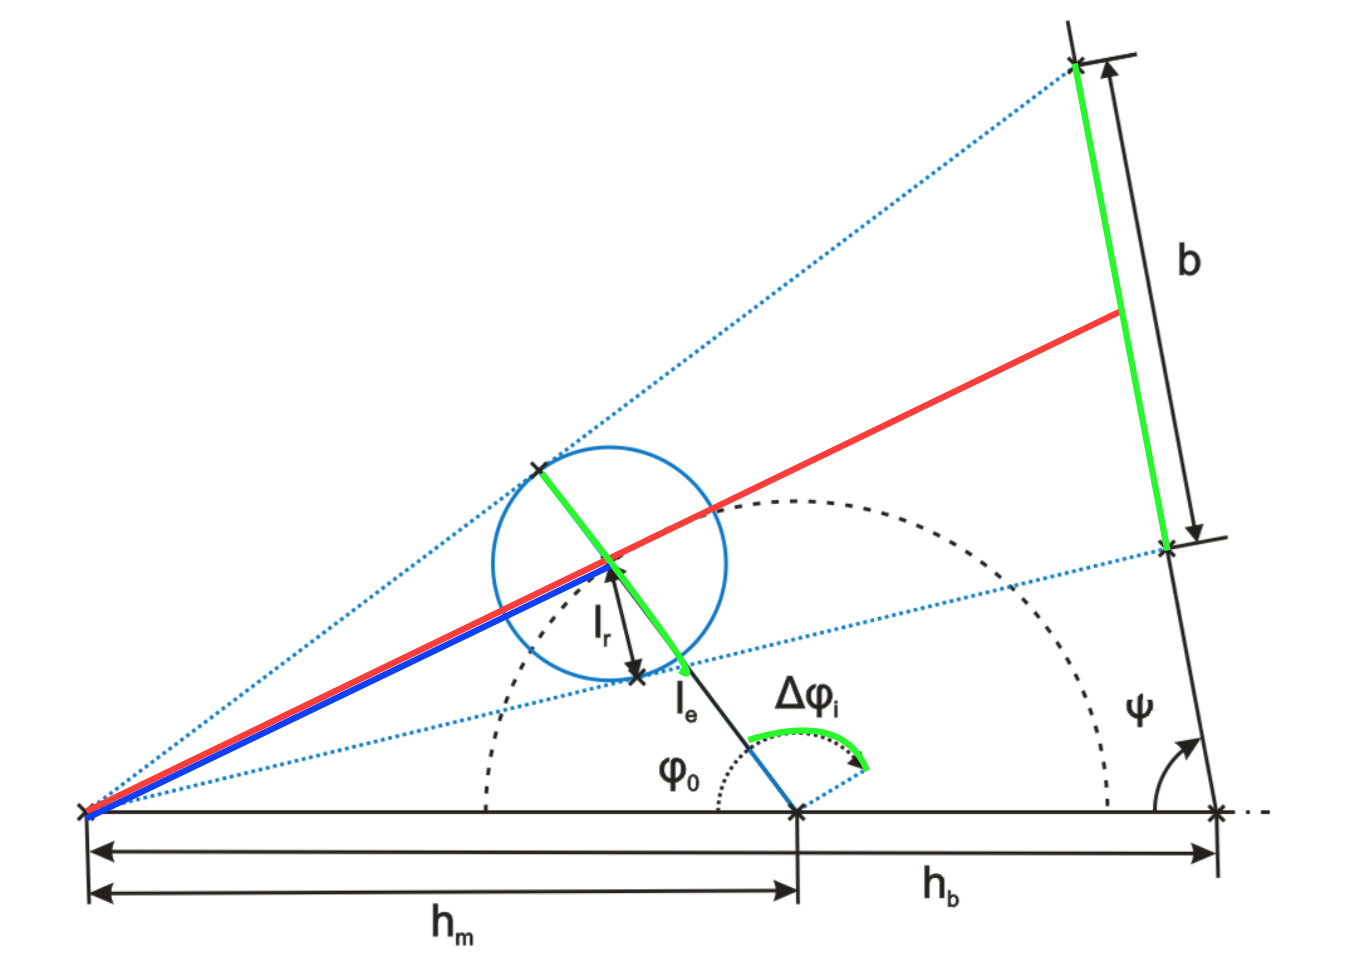
\includegraphics[width=\linewidth]{images/raw.png}
		\end{column}
		\begin{column}{0.3\linewidth}
			\begin{itemize}
				\item bekannt:
				\begin{itemize}
					\item b
					\item $l_r$
					\item $\Delta \phi_i$
				\end{itemize}
				\item unbekannt: x
				\begin{itemize}
					\item $\phi_0$
					\item $l_e$
					\item $h_m$
					\item $h_b$
					\item $\psi$
				\end{itemize}
			\end{itemize}
		\end{column}
	\end{columns}
\end{frame}

\begin{frame}{Geometrie}
	\begin{columns}
		\begin{column}{0.68\linewidth}
			\centering
			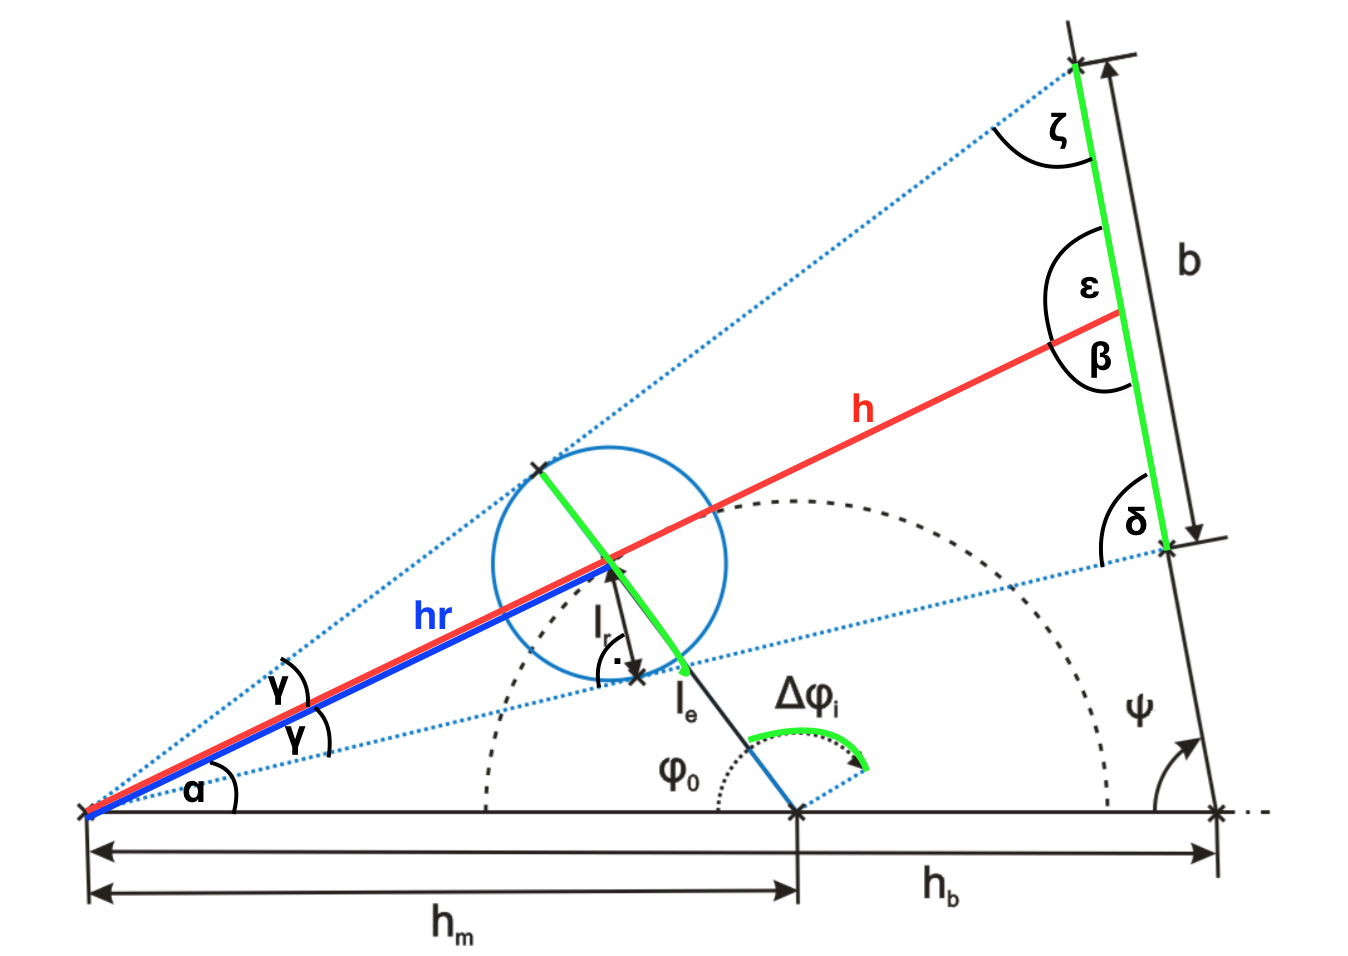
\includegraphics[width=\linewidth]{images/edited.png}
		\end{column}
		\begin{column}{0.3\linewidth}
			\begin{itemize}
				\item bekannt:
				\begin{itemize}
					\item b
					\item $l_r$
					\item $\Delta \phi_i$
				\end{itemize}
				\item unbekannt: x
				\begin{itemize}
					\item $\phi_0$
					\item $l_e$
					\item $h_m$
					\item $h_b$
					\item $\psi$
				\end{itemize}
			\end{itemize}
		\end{column}
	\end{columns}
\end{frame}

\section{Berechnung}
\subsection{Erinnerung}
\begin{frame}{Sinus- und Kosinussatz}
	Sinussatz:
	\begin{align*}
	\frac{a}{sin \alpha} = \frac{b}{sin \beta} = \frac{c}{sin\gamma}
	\end{align*}
	Kosinussatz (b, c analog):
	\begin{align*}
	a^2 = b^2 + c^2 - 2bc\cdot cos\alpha\\
	\end{align*}
\end{frame}

\subsection{Formeln}
\begin{frame}{explizite Formel}
	$$ \mbox{ \fontsize{4pt}{2} $
	\begin{split}
	b (l_r, l_e, h_m, h_b, \phi, \psi) =\\ 
	\bigg[\frac{1}{- \sqrt{1 - \left(\frac{l_r}{\sqrt{l_e^2 + h_m^2 - 2l_eh_m\cdot cos(\phi)}}\right)^2} + cos(2 * arcsin(\frac{l_e * sin(\phi)}{\sqrt{l_e^2 + h_m^2 - 2l_eh_m\cdot cos(\phi)}}) + 2 * \psi - arcsin(\frac{l_r}{\sqrt{l_e^2 + h_m^2 - 2l_eh_m\cdot cos(\phi)}}))}\\ 
	+ \frac{1}{\sqrt{1- \left(\frac{l_r}{\sqrt{l_e ^2 + h_m^2 - 2*l_e*h_m * cos(\phi)}}\right)^2} - cos(2*arcsin(\frac{l_e * sin(\phi)}{\sqrt{l_e ^2 + h_m^2 - 2*l_e*h_m * cos(\phi)}}) + 2* \psi - arcsin(\frac{l_r}{\sqrt{l_e ^2 + h_m^2 - 2*l_e*h_m * cos(\phi)}}))}\bigg]\\
	\cdot\bigg(2 * \frac{l_r}{\sqrt{l_e ^2 + h_m^2 - 2*l_e*h_m * cos(\phi)}} * sin(\phi) * h_b\bigg)
	\end{split} $}$$
\end{frame}

\begin{frame}{Herleitung}
	\begin{columns}
		\begin{column}{0.55\linewidth}
			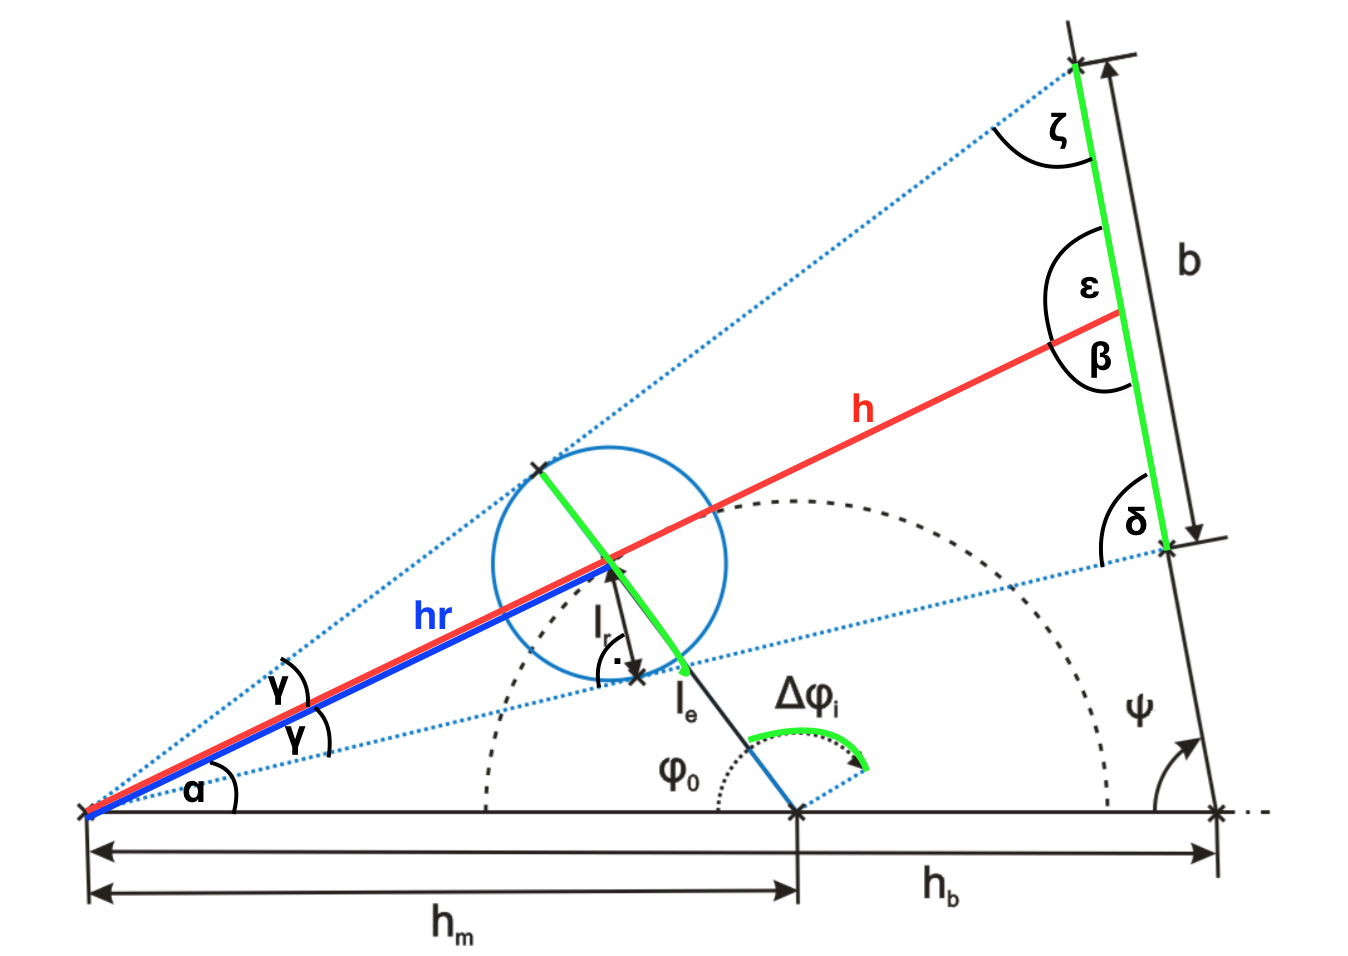
\includegraphics[width=\linewidth]{images/edited.png}
		\end{column}
		\begin{column}{0.43\linewidth}
			$$ \mbox{ \footnotesize $ \begin{align}
				h_r = \sqrt{l_e^2 + h_m^2 - 2l_eh_m\cdot cos(\phi)}\\
				\alpha =arcsin\left(l_e \cdot \frac{sin(\phi)}{h_r}\right)\\
				\beta = \pi - \alpha - \psi\\
				h = sin(\phi) \cdot \frac{h_b}{sin(\beta)}\\
				\gamma = arcsin(\frac{l_r}{h_r})\\
				\delta = \pi - \beta - \gamma\\
				b_{bottom} = \frac{sin(\gamma)}{sin(\delta)}\cdot h\\
				\epsilon = \pi - \beta\\
				\zeta = \pi - \epsilon - \gamma\\
				b_{top} = \frac{sin(\gamma)}{sin(\zeta)}\cdot h\\
				b = b_{top} + b_{bottom}
				\end{align} $} $$
		\end{column}
	\end{columns}
\end{frame}

\section{Implementierung}
\subsection{Vorwärtsproblem}
\begin{frame}{Vorwärtsproblem}
	\begin{itemize}
		\item alles bekannt, berechne Schattenbreite
		\item direkte Implementierung der Herleitung
		\item Plots und Prints zum Verifizieren
	\end{itemize}
	\centering
	\vspace{0.2cm}
	Live-Vorführung\\
	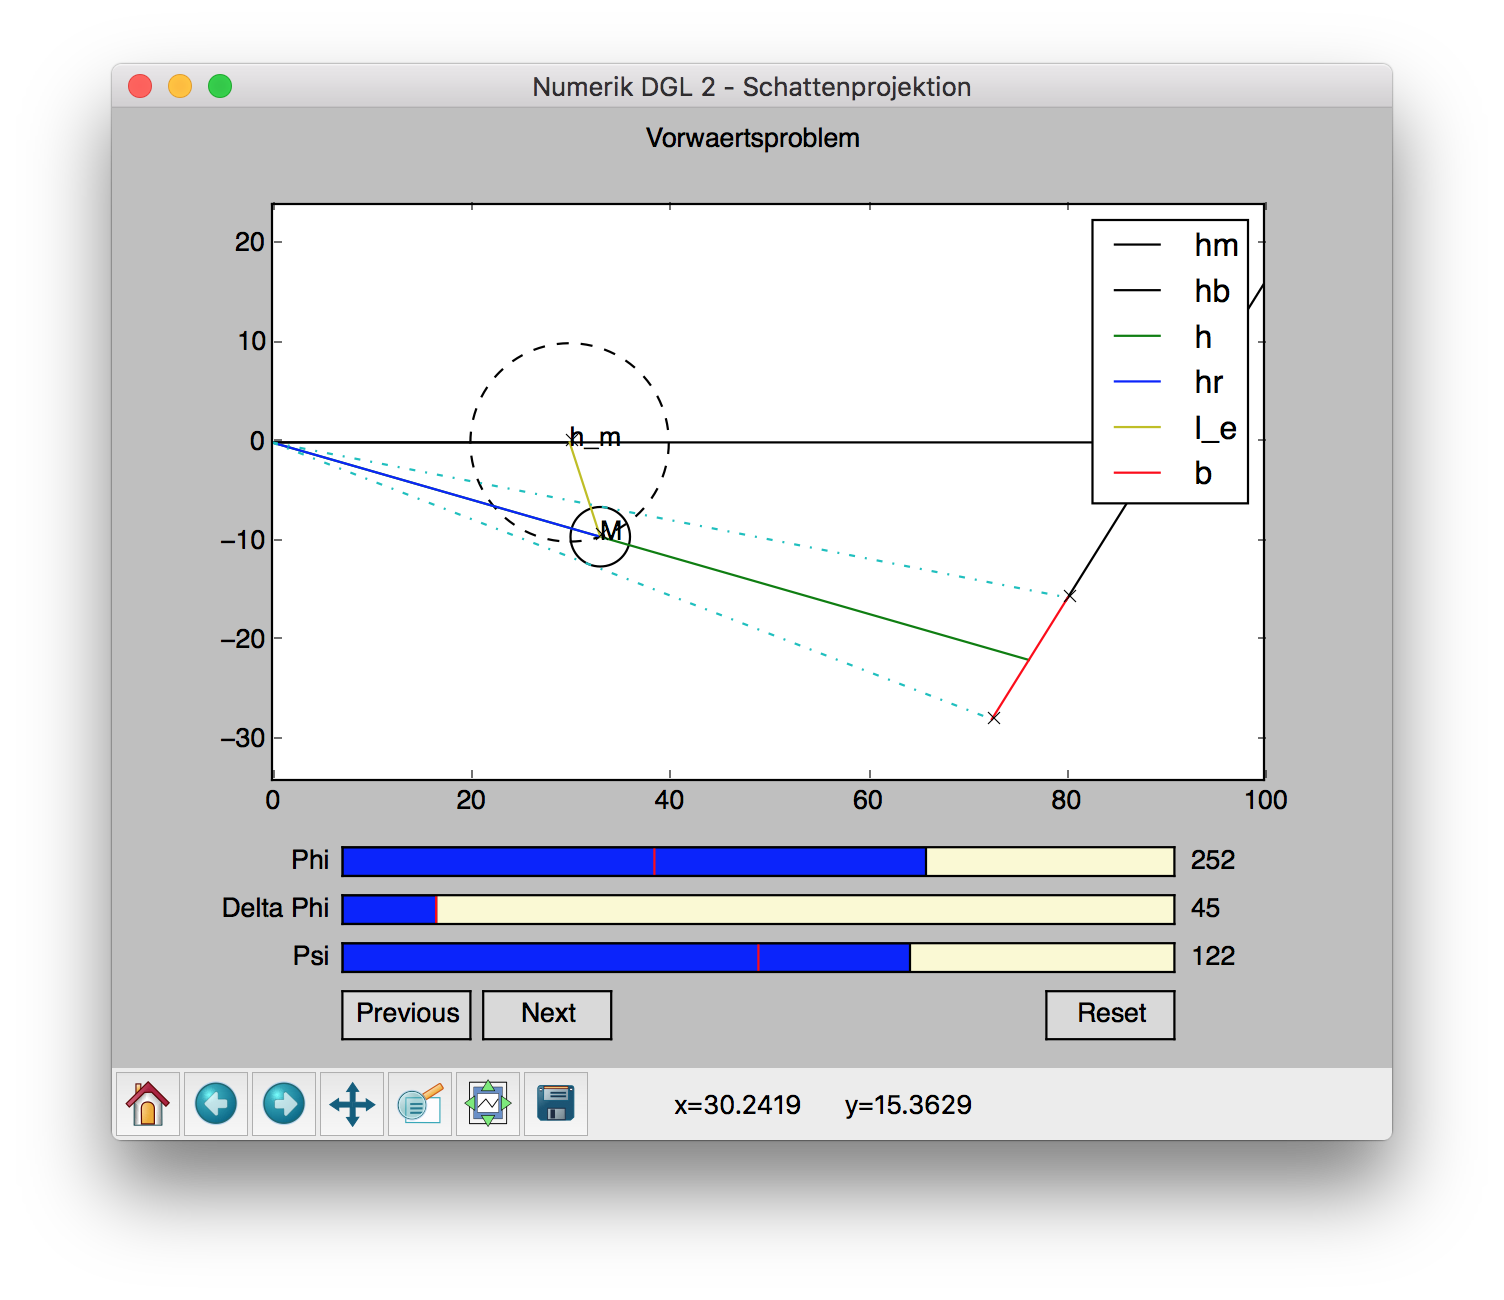
\includegraphics[width=0.6\linewidth]{images/vorfuehrung.png}
\end{frame}

\subsection{Rückwärtsproblem}
\begin{frame}{Rückwärtsproblem}
	\begin{itemize}
		\item bekannt: Schattenbreite, Radius vom Zylinder und Drehwinkel
		\item berechne: x
		\vspace{0.4cm}
		\item Gauß-Newton-Verfahren
		$$x_{k+1} = x_k − F′(x_k)^+F(x_k)$$
	\end{itemize}
\end{frame}

\begin{frame}{Regularisierung}
	\begin{itemize}
		\item Regularisierung mit Tikhonov
	\end{itemize}
	\begin{align}
		R_\alpha =(A^TA+\alpha I)^{-1}A^T\\
		x_\alpha = R_\alpha y \Rightarrow (A^TA+\alpha I)x_\alpha =A^Ty
	\end{align}
	\begin{itemize}
		\item adaptive Steuerung vom $\alpha$ zur Konvergenzbeschleunigung
	\end{itemize}
\end{frame}

\begin{frame}{Live-Demo}
	\centering
	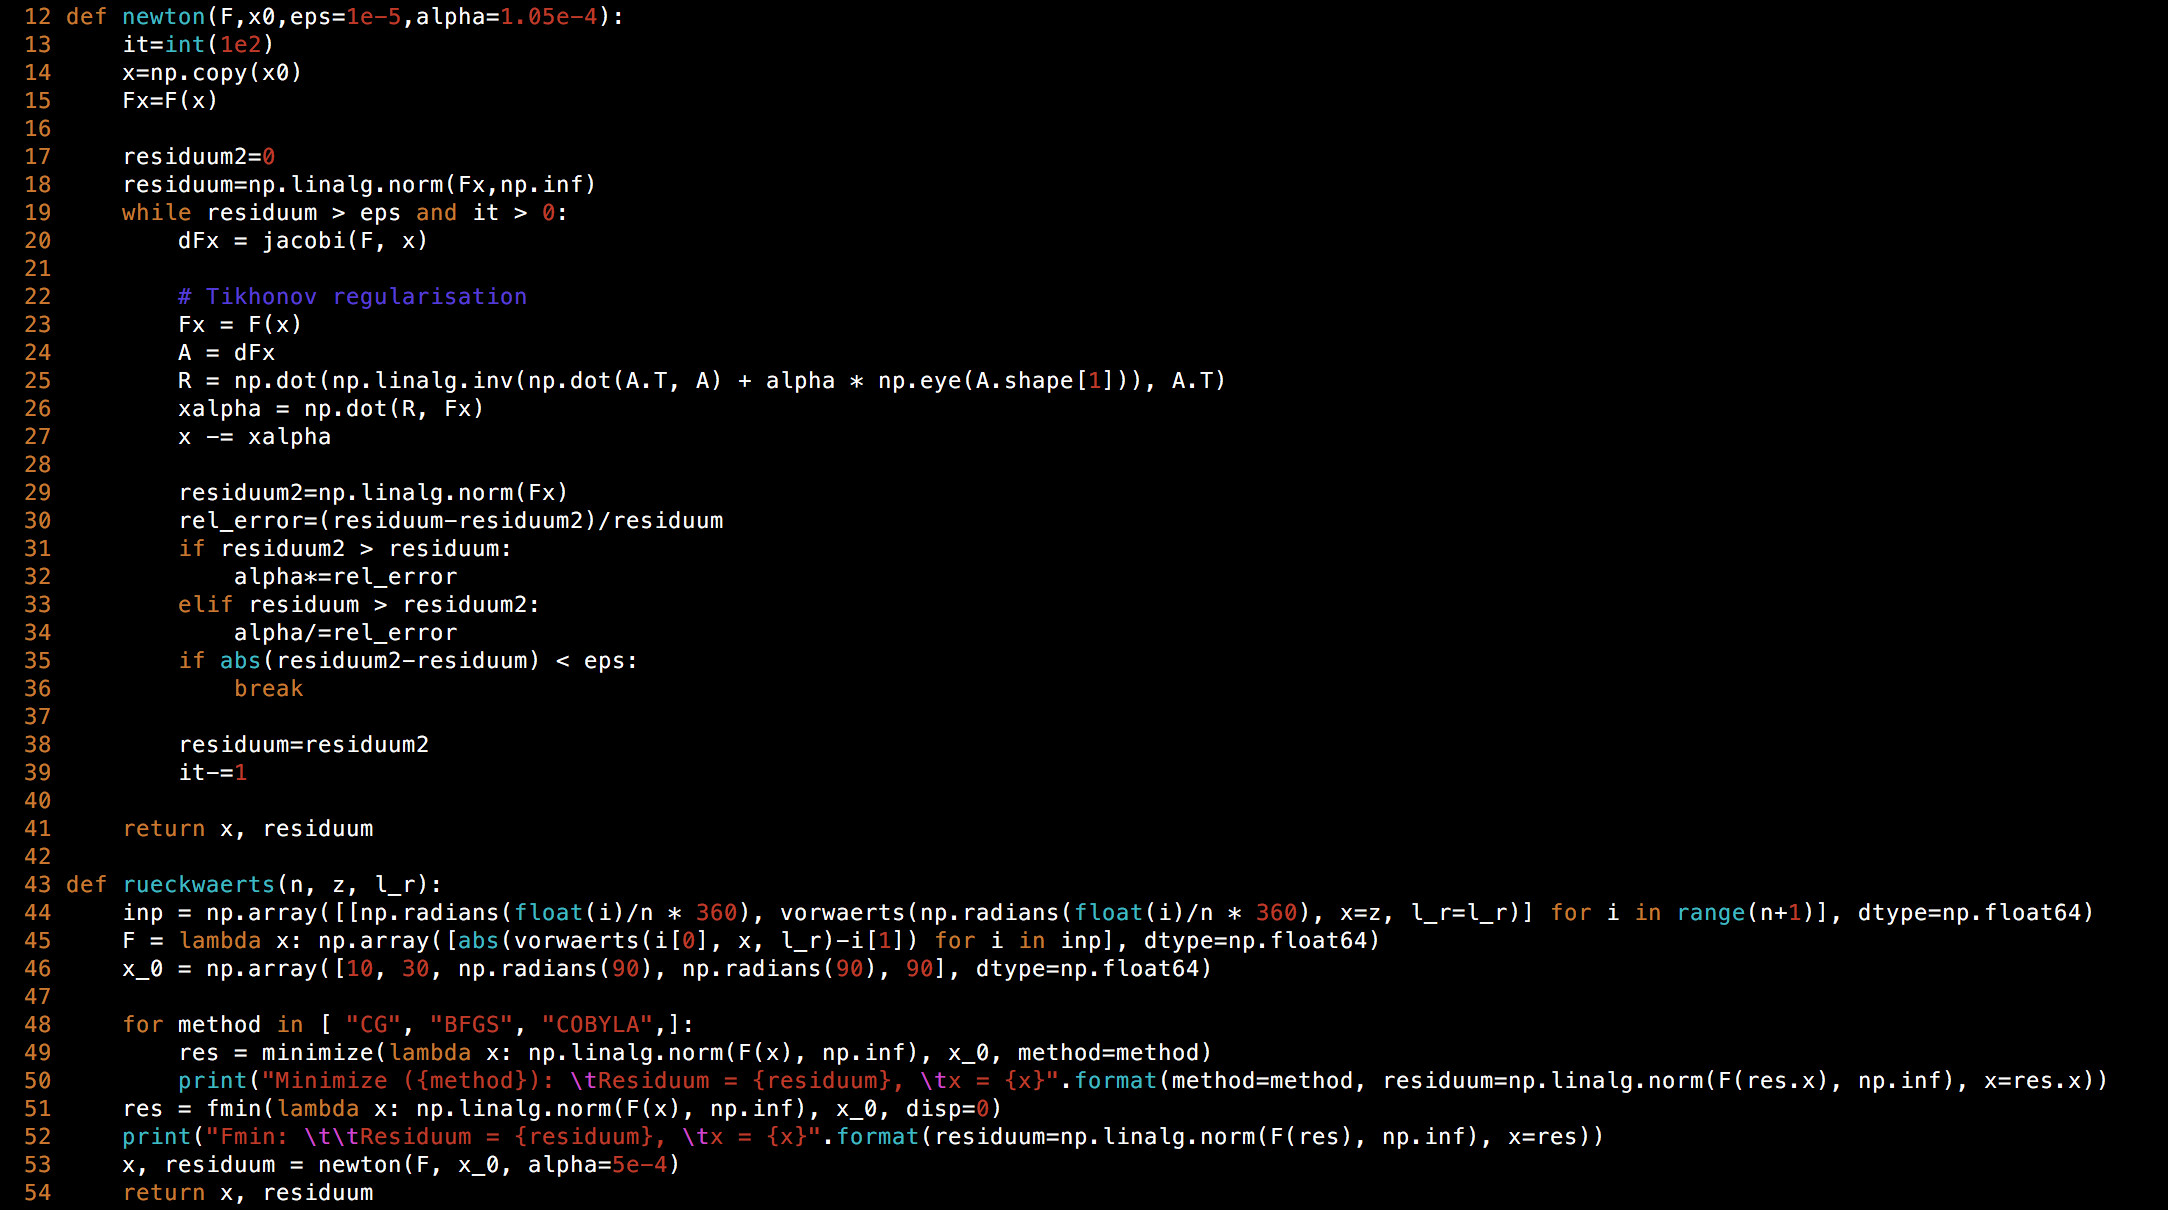
\includegraphics[width=\linewidth]{images/quellcode.png}
\end{frame}

\section{Ende}
\begin{frame}{Ende}
	\centering
	Vielen Dank für Eure Aufmerksamkeit.
\end{frame}
\end{document}	